\documentclass{article}[12pt]

%--------------Packages------------------------------
\usepackage[utf8]{inputenc} %Pour encoder du texte en français
\usepackage[francais]{babel} %Pour encoder du texte en français
\usepackage{graphicx} %pour inclure des images
\usepackage{changepage}
\usepackage{version} % permet d'utiliser l'environnement comment
\graphicspath{{./figures/}} %repertoire images
\usepackage{listings} %si on veut afficher du code, le code doit se trouver dans un dossier "codes" 					  %lui même dans le même répertoire que ce fichier tex
\usepackage{color} %nécessaire pour changer les couleurs du highlighting du code
\usepackage{amsmath,amssymb}%pour des maths au cas où
\usepackage{array,multirow,makecell}%Pour manipuler les tableaux
\usepackage{url} %pour utiliser les liens hypertextes
\usepackage{hyperref} %pour utiliser les liens hypertextes
\usepackage{float}
\newlength{\offsetpage}
\setlength{\offsetpage}{2.0cm}
\usepackage[left=2cm,right=2cm,top=2cm,bottom=2cm]{geometry}
\newenvironment{widepage}{\begin{adjustwidth}{-\offsetpage}{-\offsetpage}%
    \addtolength{\textwidth}{2\offsetpage}}%
{\end{adjustwidth}}

\newcommand{\Java}[2]{
	\begin{itemize}
    	\item[]\lstinputlisting[caption=#2,label=#1]{#1.java}
	\end{itemize}
}
% ---------- Document ------------ %
\begin{document}

\begin{titlepage}

\newcommand{\HRule}{\rule{\linewidth}{0.5mm}} % Defines a new command for the horizontal lines, change thickness here

\center % Center everything on the page
 
%----------------------------------------------------------------------------------------
%	HEADING SECTIONS
%----------------------------------------------------------------------------------------

\textsc{\LARGE Institut Paul Lambin}\\[1.5cm] % Name of your university/college
\textsc{\Large BAC 2 Informatique de gestion}\\[0.5cm] % Major heading such as course name
\textsc{\large Unix}\\[0.5cm] % Minor heading such as course title

%----------------------------------------------------------------------------------------
%	TITLE SECTION
%----------------------------------------------------------------------------------------

\HRule \\[0.4cm]
{ \huge \bfseries Synthèse Unix }\\[0.4cm] % Title of your document
\HRule \\[1.5cm]
 
%----------------------------------------------------------------------------------------
%	AUTHOR SECTION
%----------------------------------------------------------------------------------------

\begin{minipage}{0.4\textwidth}
\begin{flushleft} \large
\emph{Auteurs:}\\
Christopher \textsc{Sacré} \\ % Your name
\end{flushleft}
\end{minipage}
~
\begin{minipage}{0.4\textwidth}
\begin{flushright} \large
\emph{Professeur:} \\
C. \textsc{De Muylder}\\
B. \textsc{Henriet}\\
A. \textsc{Ninane}% Supervisor's Name

\end{flushright}
\end{minipage}\\[4cm]

% If you don't want a supervisor, uncomment the two lines below and remove the section above
%\Large \emph{Author:}\\
%John \textsc{Smith}\\[3cm] % Your name

%----------------------------------------------------------------------------------------
%	DATE SECTION
%----------------------------------------------------------------------------------------

{\large \today}\\[3cm] % Date, change the \today to a set date if you want to be precise

%----------------------------------------------------------------------------------------
%	LOGO SECTION
%----------------------------------------------------------------------------------------

%\includegraphics{Logo}\\[1cm] % Include a department/university logo - this will require the graphicx package
 
%----------------------------------------------------------------------------------------

\vfill % Fill the rest of the page with whitespace

\end{titlepage}

\tableofcontents%table des matières
\newpage
\section{Schémas vus au cours}
\subsection{Semaine 2}
\subsubsection{Diagramme}
\begin{figure}[H]
	\fbox{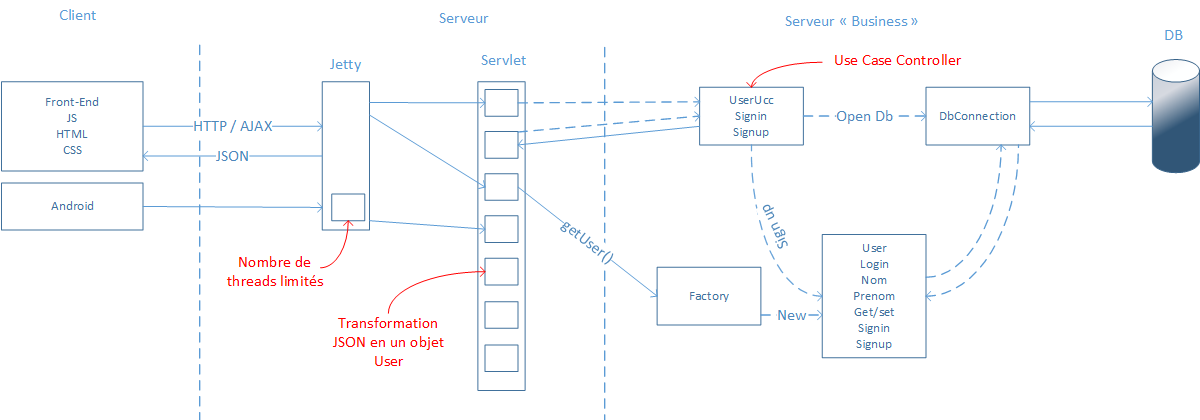
\includegraphics[scale=0.53]{Schema_2.png}}
    \centering
    \caption{Introduction du cours}
\end{figure}
\subsubsection{Informations supplémentaires : }
Si vous souhaitez des informations supplémentaires, plusieurs logiciels ont été mentionné durant ce cours : Harmony, Visual Studio Code ainsi que Electron. (Il s'agit d'un cours nous introduisant les concepts de notre application ainsi que les bases de son architecture).
\subsection{Semaine 3}
\subsubsection{Diagramme}
\begin{figure}[H]
	\fbox{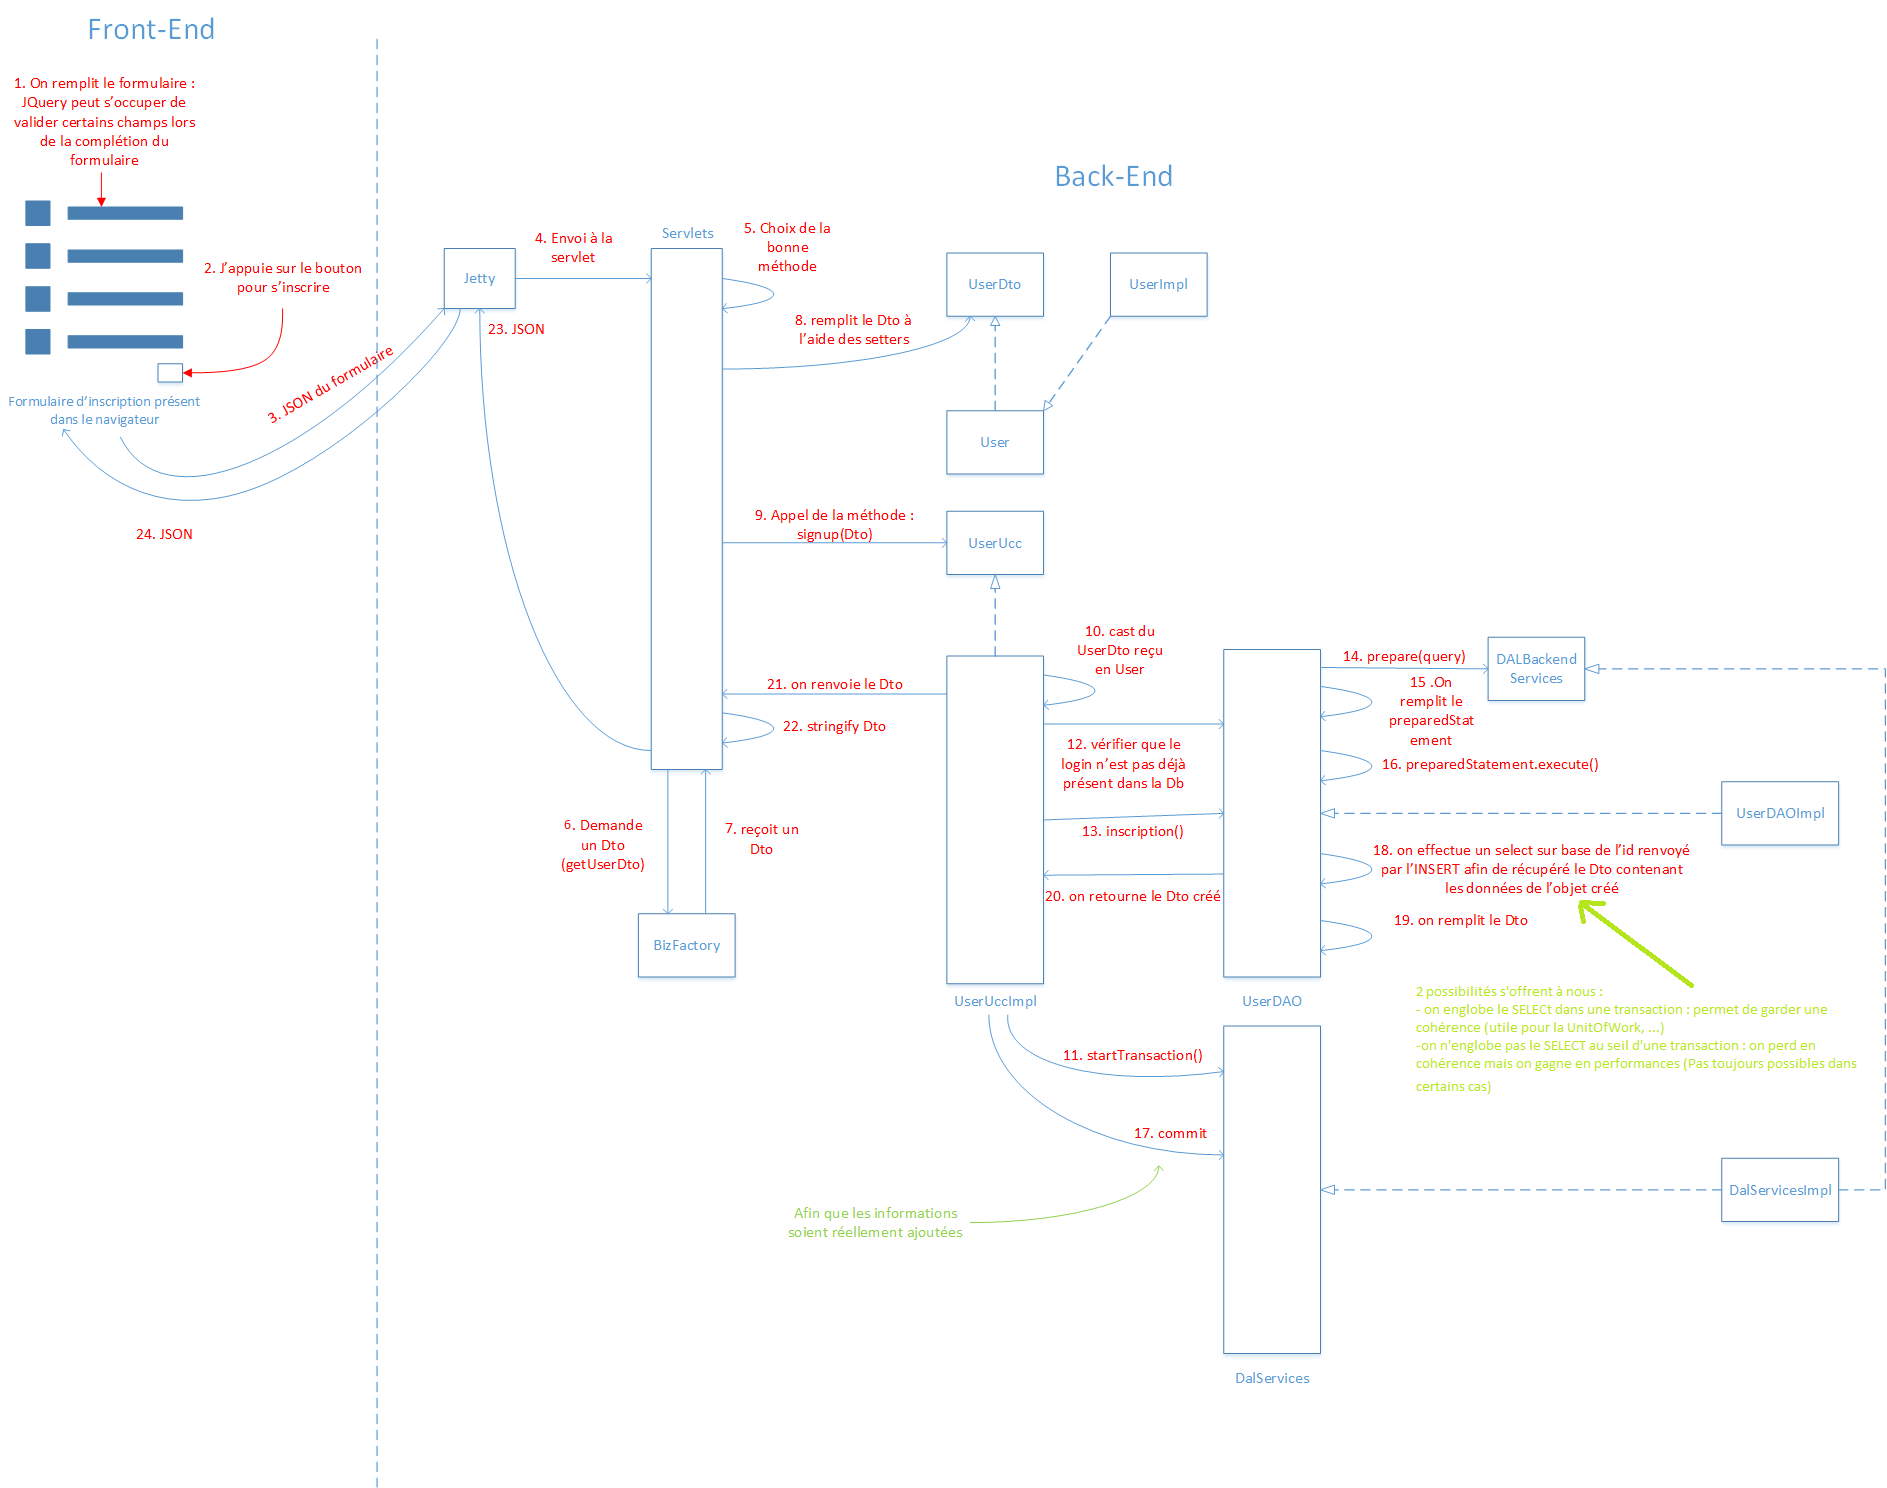
\includegraphics[scale=0.35]{Schema_3.png}}
    \centering
    \caption{Exemple d'utilisation de notre architecture (UC : s'inscrire)}
\end{figure}
\subsection{Semaine 4}
\subsubsection{Diagramme}
\begin{figure}[H]
	\fbox{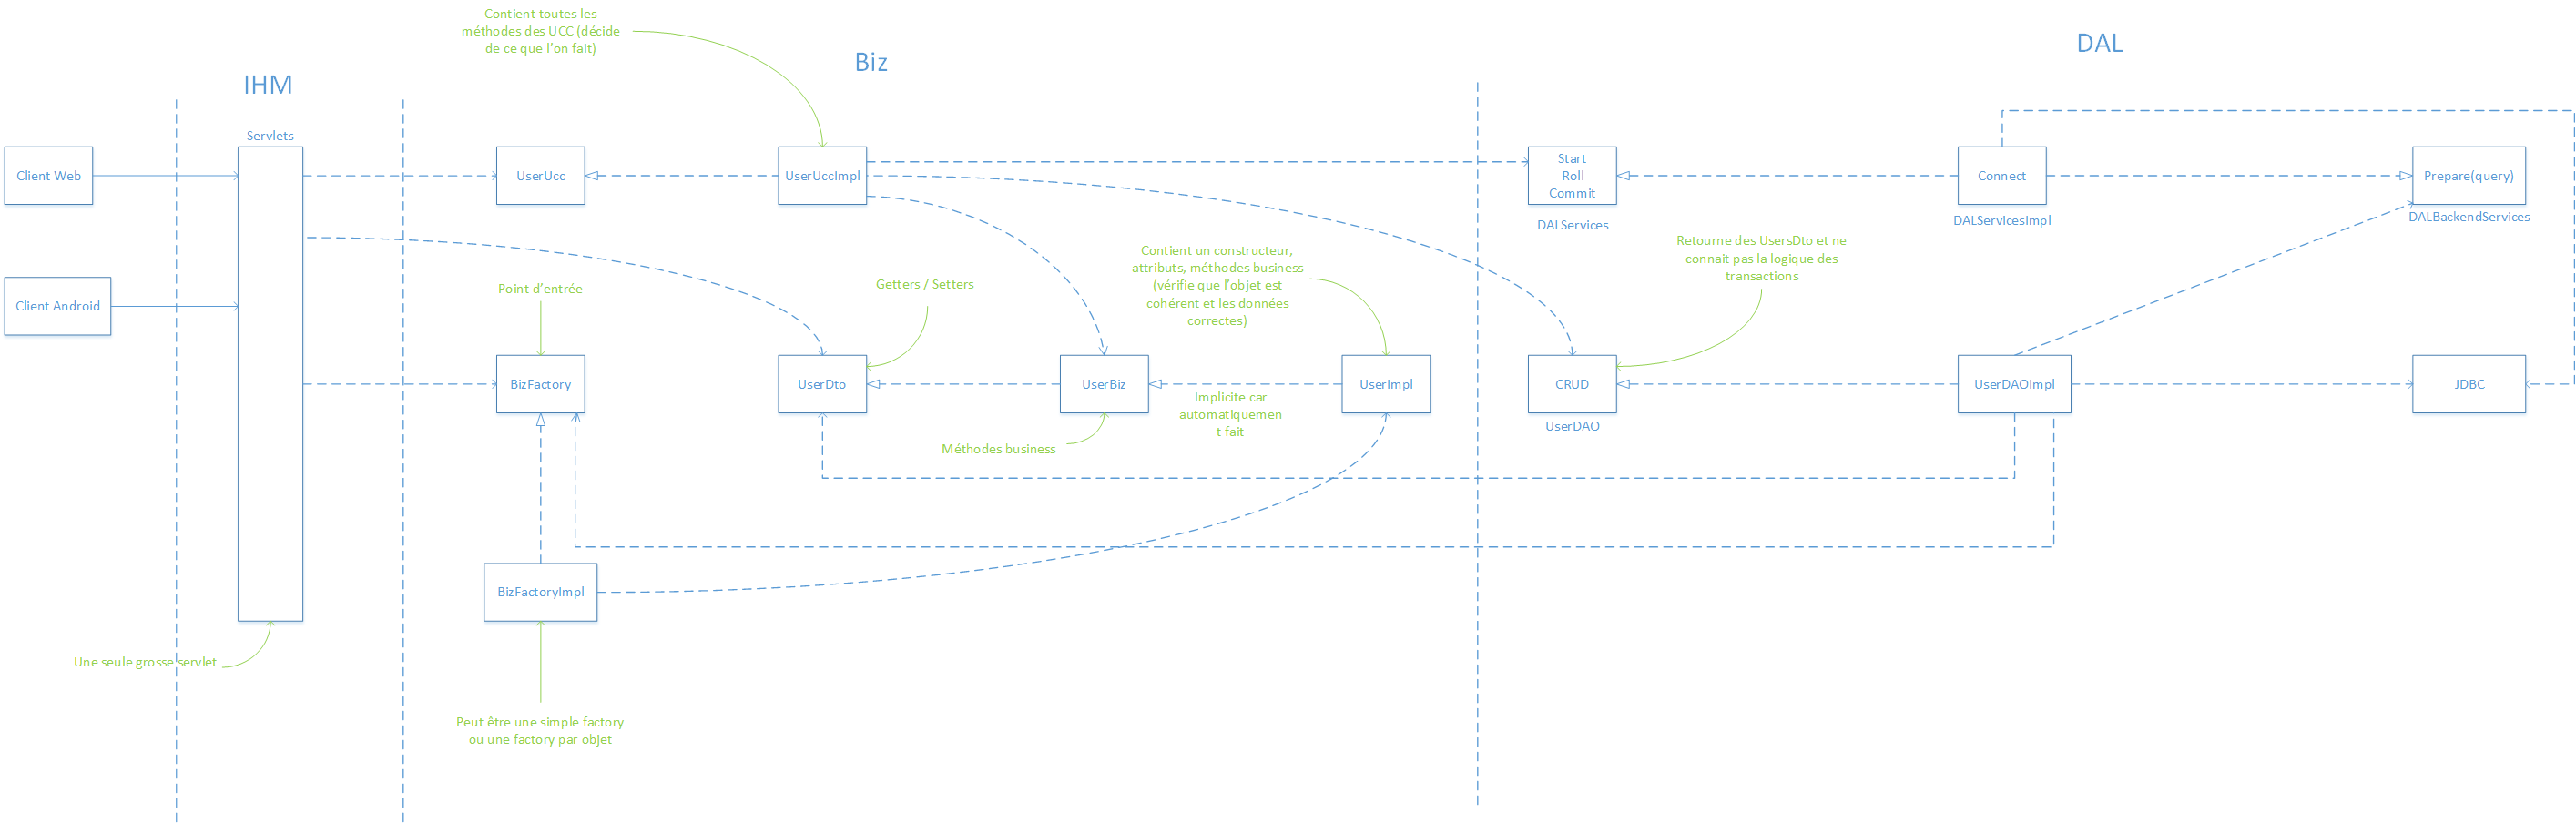
\includegraphics[scale=0.25]{Schema_4.png}}
    \centering
    \caption{Architecture Monothread complète}
\end{figure}
\subsubsection{Informations suppémentaires : } 
\paragraph{Factoring : } Il faut savoir que l'on mettra de nombreuses classes, ... public mais on tentera d'utiliser uniquement les points d'entrées (surtout au sein de la couche IHM), dans le même style, on utilisera de nombreuses interfaces afin de diminuer le nombre de dépendances concrètes et faciliter le changement entre l'environnement de prod et celui de dev. Par ailleurs, la servlet ne doit pas connaitre les méthodes bussiness (Car dans le cas contraire elle pourrait les modifier). 
\paragraph{Traitement des INSERT : }lorsque l'on insère, on tente de retourner l'entièreté de l'objet crée et non juste l'id, cela permet de vérifier que tout c'est bien passé. 
\paragraph{Traitement des SELECT : } point suivant est plutôt controversé et dépend de votre version des choses il s'agit de l'utilisation de transactions au niveau des select : on peut ne pas utiliser de transaction (perte de cohérence mais gain de performances) ou au contraire utiliser des transactions (perte de performances mais gain de cohérence). 
\paragraph{Sécurité : } Il est important que le back-end soit totalement indépendant du front-end (les données reçues ne sont en aucun cas sure).
\paragraph{Remarque : } un framework nous pose des rails, cela nous permet uniquement de nous orienter , dès lors il faut parfois s'éloigner des rails.
\subsection{Semaine 5}
\paragraph{Main : } Le main permet de démarrer Jetty, c'est lui qui s'occupe de créer les servlets Jetty. Il crée les Factory à l'ai de l'injection de dépendance. Dés que tout cela est créé, il se met en pause (Le main se lance au démarrage de l'application).
\subsection{Semaine 6}
\subsubsection{Diagramme}
\begin{figure}[H]
	\fbox{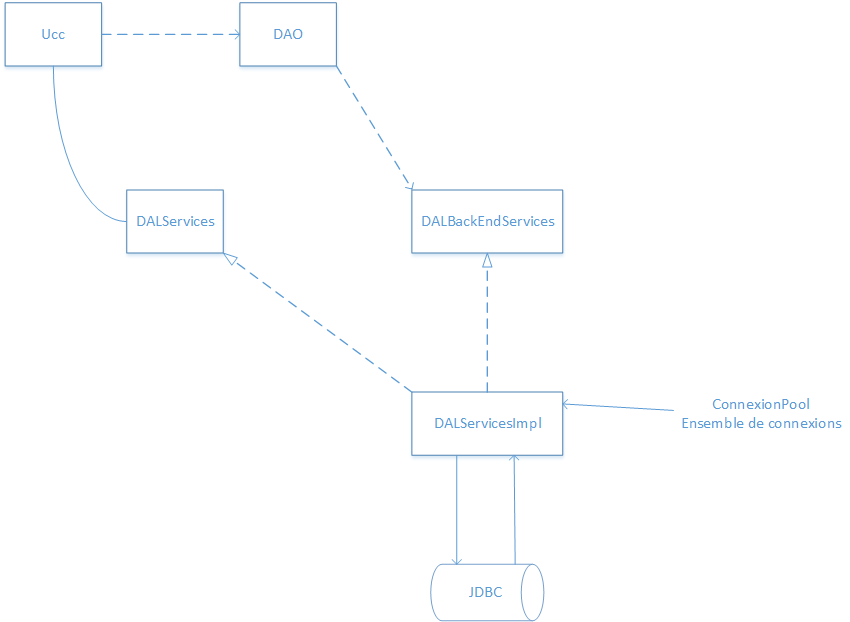
\includegraphics[scale=0.50]{Schema_5.png}}
    \centering
    \caption{Connexion Pool}
\end{figure}
\subsubsection{Informations}
\paragraph{Introduction : } gros problème que l'on a tenté de résoudre est le fait que l'on ne pouvait ouvrir qu'une seule transaction à la fois (Il est totalement interdit d'ouvrir plusieurs transactions sur la même connexion en même temps, En cas de transactions imbriquées, si la première transaction à un soucis le rollback ne se propagera pas, mais s'arrêtera au premier commit). 
\paragraph{Solution : } Jetty à pour cela, un ensemble de Thread (Il n'en a pas un nombre infinis). On va donc remplacer notre précédente unique connexion par un ensemble de connexions (Le nombre de connexions à avoir est de notre ressort, et c'est donc à nous de faie ce choix).
\paragraph{Aide à la solution : } On peut afin de nous aider à implémenter cela utiliser ThreadLocal (On aurait dès lors une connexion par thread, utilisation d 'une Map<Thread, ConnexionDb> (pour cela on peut utiliser la méthode Thread.getId() qui renvoie l'id du threadCourant), ou plus facile encore ou pourrait utiliser la classe ThreadLocal, notre Map deviendrait alors un ThreadLocal<Connexion>, la clé est directement l'id du thread local (il s'agit tout simplement d'une map pour laquelle on a spécifié la syntaxe)). 
\paragraph{Problème : } le problème avec ces deux solutions vient du fait que si il y a une connexion par thread, on va donc multiplier le nombre de connexions (La taille du threadPool est un problème en soit (il faut pouvoir la fixer et cela dépend la plupart du temps fort de la couche Bussiness (Si il n'y a pas assez de Connexions, cela bloquera le thread tant qu'il n'y en aurait pas une de disponible). 
\paragraph{Solution Finale : } Afin de palier à tout cela, on va utiliser DBCP2 (Une librairie Java, DataBaseConnexionPool).
\subsection{Semaine 7}
\subsubsection{Informations}
\paragraph{Affichage des erreurs : } Afin d'afficher des erreurs on peut utiliser System.err.println (La différence avec System.out.println est qu'il pourrait y avoir un décallqge au niveau de l'affichage).
\paragraph{Classe Logger : } La classe Logger permet de définir une priorité au niveau des messages (Il plusieurs niveaux de priorité : SEVERE (valeur la plus élevée), WARNING, INFO, CONFIG, FINE, FINER, FINEST (valeur la moins élevée). L'avantage de cela est que l'on pourrait Logger sur un autre serveur , permettant ainsi d'empêcher la surcharge d'un appareil (Il est intéréssant de Logger : le temps de réponse, le type d'appareil utilisé , le type de route utilisé, ou tout ce qui vous semble intéressant d'être connus). 
\paragraph{Profiler - SQL : } permet de connaitre le temps d'exécution d'une réponse.
\paragraph{Sécurité : } On pourrait rajouter une couche afin d'empêcher les attaques DDOS (Cette couche permettrait de filtrer les requêtes et de les dispatcher à des serveurs plus petit qui traiteraient alors les requêtes).  Un autre point important pour la sécurité est qu'il ne faut jamais faire confiance à l'utilisateur, Il faut par ailleurs faire la distinction entre Admin et Utilisateur et utiliser JWT (cf cours de JavaScript).

\end{document}
